\part{ÉTAT DE L’ART}
\chapter{PRÉSENTATION DU PROJET}

\textit{Dans ce premier chapitre de la première partie de notre mémoire, nous allons présenter
	notre projet, du contexte à la problématique sans bien sûr oublier les méthodes. Il présente
	notre projet dans son ensemble, il présente la délimitation du sujet, les problèmes à résoudre,
	l’intérêt du sujet et une étude de l’existant.}

\clearpage

\section{Compréhension du sujet}

\subsection{Context}

L’apprentissage est un ensemble de mécanismes menant à l'acquisition de savoir-faire, de savoirs ou de connaissances afin de s’en servir dans la vie courante ou de les faire évoluer pour les générations futures. Malgré les évolutions technologiques offrant de nouvelle façon d’acquérir des connaissances, le système éducatif africain plus précisément camerounais n’a pas beaucoup évoluer les moyens de dispenser les connaissances ne suivent pas toujours les tendances actuelles. Les personnes apprennent mieux en s’immergent dans ce qu’ils font qu’en le théorisant, cela est toujours possible dans le processus d’apprentissage mais pas dans tous les domaines de formation du fait des risque lié à l’acquisition des connaissances en pratique.

Parmi ces domaines ou l’immersion réel des apprenant dans les conditions réels de pratique présente des risques réel pour l’apprenant nous pouvons parler de la chimie, qui est un domaine de la science très expérimentale nécessitant des observations pour une compréhension du sujet étudié en vue d’y apporter des applications dans la vie courante. Une grande et bonne compréhension de ce domaine pourrait apporter de nombreuses idées de recherche qui permettront des avancées significatives dans de nombreux domaines (agriculture, industrie, mode, la mécanique, l'énergie…), avancées qui pourraient à leur tour faciliter le processus d'émergence en Afrique et plus précisément au Cameroun. Malgré l’aspect très expérimentale de son apprentissage, il reste assez dangereux et couteux à enseigner en pratique, dangereux car le manque d’expérience des apprenant pourrais les pousser à commettre des erreurs qui pourrait causer des accidents très dangereux voire mortelle en fonction des éléments manipulés et couteux car la maintenance du matériel nécessaire aux expérimentations (local, verrerie, éléments et personnelles de maintenance) engendre des coûts assez élevé.

\textbf{VREDU} est une plateforme dont l’objectif est de limiter les coûts et les risques lors des expérimentations en concevant le réalisme afin de créer un sentiment d’immersion pour une meilleure compréhension. Pour ce faire monglo technology s’est intéressé à la réalité virtuelle qui est une expression désignant les dispositifs permettant de simuler numériquement un environnement par la machine (ordinateur), afin d’apporter ce réalisme et limiter les risques d’accident.

\subsection{Délimitation du sujet et hypothèse du travail}

Notre travail se limitera au cas de la chimie.

\begin{itemize}
	\item Création des réactions chimique
	\item Expérimentation des réactions dans un environnement immersif
\end{itemize}

\subsection{Étude de l’existant}

L’étude de l’existant a pour but d'approfondir l'analyse des axes innovants d'un projet au cours d'élaboration, et avant sa mise en œuvre. Cette étude préalable sert à donner un aperçu sur la pertinence du projet, sa faisabilité ainsi que sa continuité.

\subsubsection{Description de l’existant}

Nous ne saurions débuter ce travail sans avoir une idée claire et précise sur l’existant quel qu’il soit. Dans la plupart des lycées, l’enseignement de la chimie suit un modèle traditionnel à savoir, cours théoriques en salle de classe au cours duquel l’apprenant découvre les principes théoriques nécessaire à la maitrise de cette science. Ensuite un cours pratique en laboratoire au cours duquel les apprenants découvrent la réalité des réaction grâce aux expérience scientifiques.


\subsubsection{Critique de l’existant}

Au cours de notre étude de l’existant, nous avons pu ressortir de nombreux problèmes liés à la réalisation des réactions dans un environnement réel, parmi lesquelles :

\begin{itemize}
	\item Les risques d’accident au cours d’expérimentation trop élevé dans un environnement réel accident qui peut s’avérer mortel suivant les éléments manipulés.
	\item Les coûts de maintenance des équipements qui avec le temps se détériore et nécessite d’être renouvelé ou entretenu régulièrement ce qui entraine des couts matériels et humain assez important.
\end{itemize}

\subsubsection{Quelques solutions existantes}

Il est question ici de noter les points forts de ces dernières et leurs points faibles afin d’ajuster nos objectifs.

\begin{itemize}
	\item \textbf{ONTOP DUO MEAC}

	      Ontop duo meac est une technologie de simulation de vol utilisé dans les écoles d’aviation utilisé par les formateurs pour mettre en pratique les aspects théoriques abordés durant les formations. En effet dans le domaine de l’aviation les simulateurs de vol comme celui-ci sont presque incontournables car en cas d’accident en condition réel dû au manque d’expérience des apprenants, les nombreuses vies seront menacées et des équipements très coûteux seront détruit.

	      Le dispositif est composé d’écran disposés à 180° autour de l’apprenant afin de simuler le point de vue d’un pilote et d’un cockpit fidèle à leur homologue réel.

	      \begin{figure}[H]
		      \centering
		      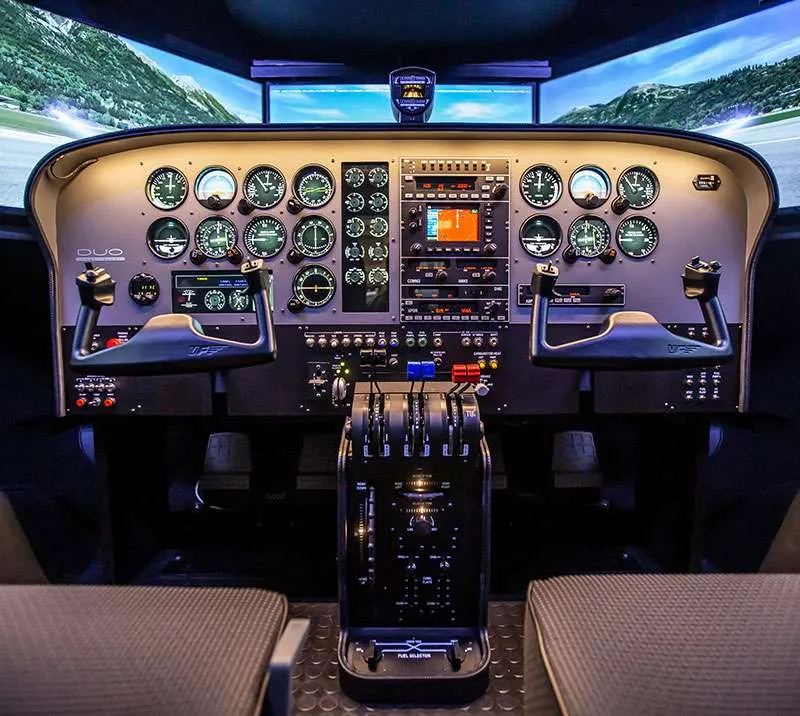
\includegraphics[width=0.5\textwidth]{img/svol1}
		      \caption{Simulateur de vol ONTOP DUO MEAC}
		      \label{fig:mesh1}
	      \end{figure}

	\item \textbf{Microsoft flight simulator}

	      Flight Simulator est un logiciel de simulation de vol pour Microsoft Windows, vendu et souvent vu comme un jeu vidéo. Tout comme le Ontop duo meac, il permet à l'apprenant de comprendre le domaine de l’aviation en pratiquant à moindre coût car il n’a besoin que d’une console de jeu (PlayStation, Xbox, ...) et de contrôleurs, ici des manettes des consoles ou des dispositifs spéciaux.

	      Cette technologie est beaucoup moins rependue dans les centres de formation, car elle est plus adaptée pour les apprenants désireux de s’entrainer chez eux et ne disposant pas des moyens pour un Ontop duo meac.

	      \begin{figure}[H]
		      \centering
		      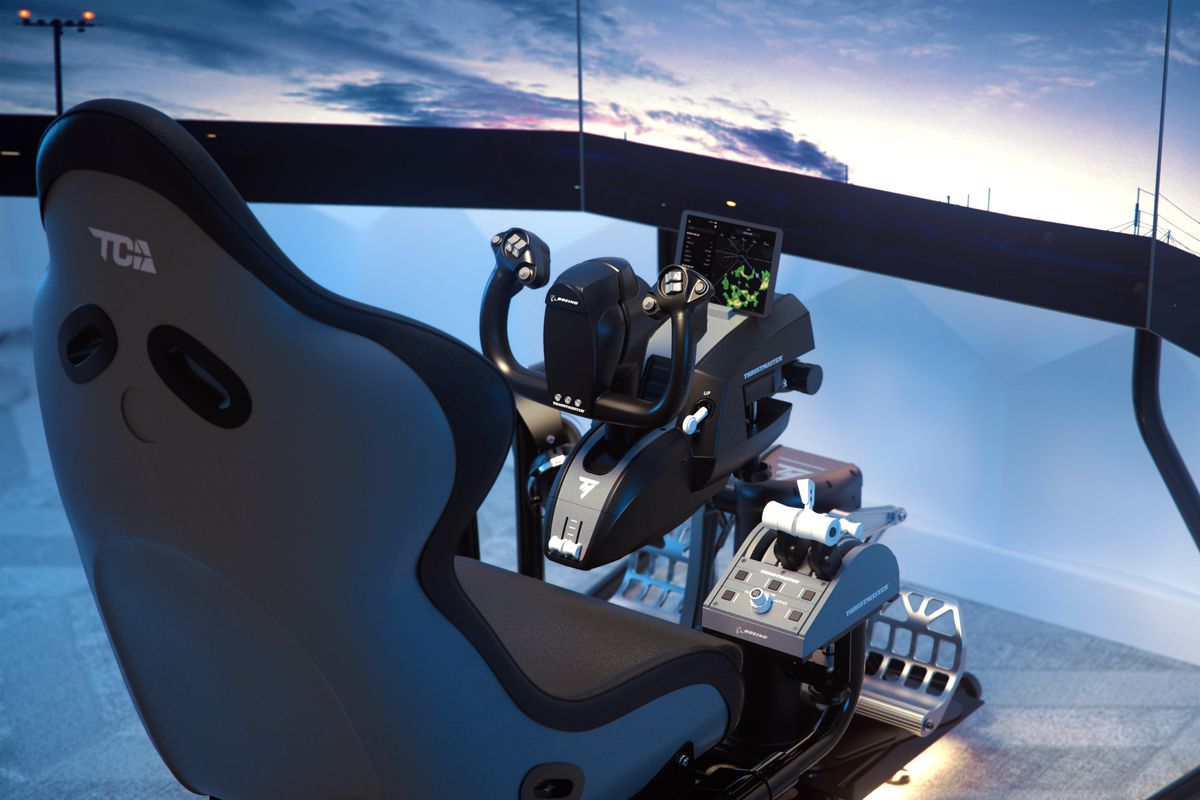
\includegraphics[width=0.5\textwidth]{img/svol2}
		      \caption{Simulateur de vol Microsoft flight simulator}
		      \label{fig:mesh1}
	      \end{figure}

	\item \textbf{Osso VR}

	      Osso VR est une plateforme de formation et d'évaluation chirurgicales qui offre aux entreprises de dispositifs médicaux et aux professionnels de la santé des moyens radicalement meilleurs de partager, de pratiquer. Tout comme dans le domaine de l’aviation, le domaine médical plus précisément chirurgicale utilise des outils de simulation de l’aspect pratique de l’apprentissage. Ceci du au risque lié à l’expérimentation sur des individue vivant et le manque de cadavre.

	      Osso VR utilise la réalité virtuelle pour les expérimentations, afin de simuler un monde en trois dimensions représentant un laboratoire ou est disposé un patient virtuel sur lequel seront effectué les expérimentations.

	      \begin{figure}[H]
		      \centering
		      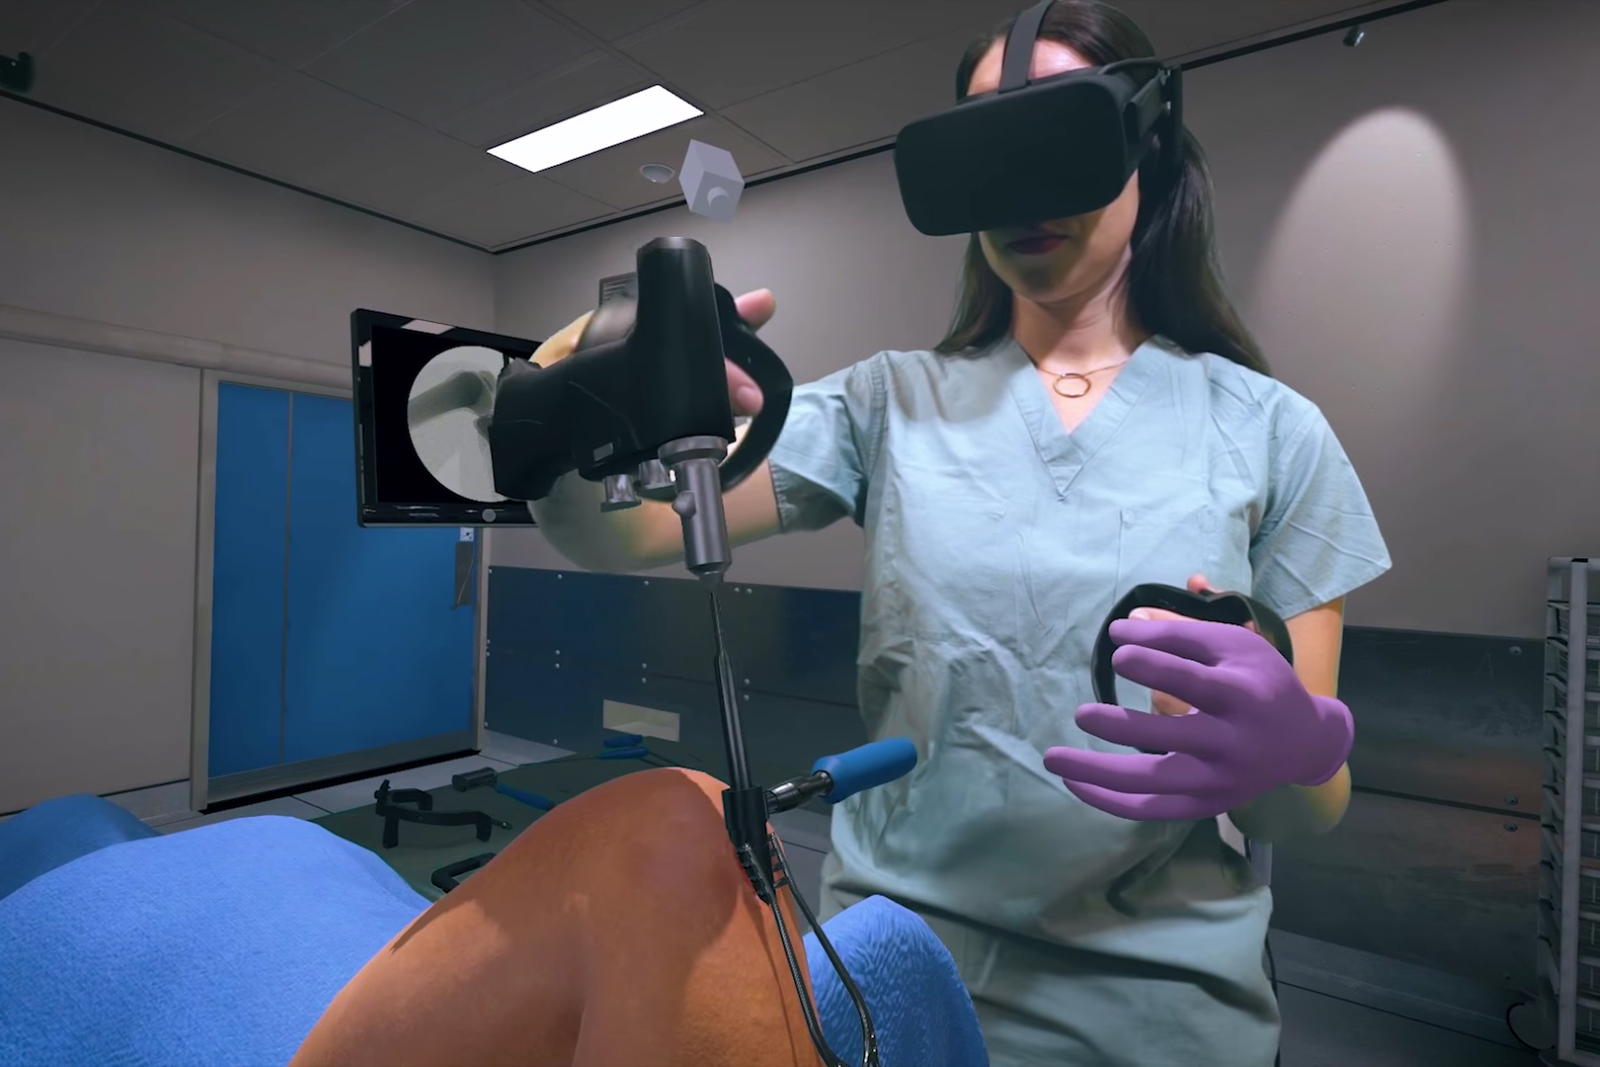
\includegraphics[width=0.5\textwidth]{img/vsurgery}
		      \caption{Simulateur chirurgicale Osso VR}
		      \label{fig:mesh1}
	      \end{figure}

	\item \textbf{Praxilab}

	      Praxilab est un outil didacticiel permettant la simulation d’expérience scientifiques dans les domaines de la biologie, la physique et la chimie. Cet outil est développé pour les plateformes desktop et web et permet aux apprenant de suivre des instructions afin de réaliser des expériences et comprendre des phénomènes liés aux différents domaines.

	      \begin{figure}[H]
		      \centering
		      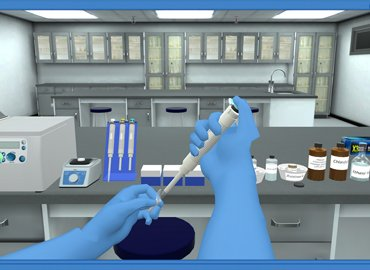
\includegraphics[width=0.5\textwidth]{img/vlab1}
		      \caption{Simulateur scientifique Praxilab}
		      \label{fig:mesh1}
	      \end{figure}

	\item \textbf{EON Reality}

	      EON Reality est une solution de formation académique et industrielle en réalité augmentée et virtuelle. Elle permet l’expérimentation virtuel dans plusieurs domaines de l’enseignement à savoir la mécanique, la chimie, la biologie, l’histoire, le génie civil et plein d’autres domaines.

	      Cette solution est disponible sur de nombreux support à savoir ordinateur sur Windows, casques de réalité virtuelle oculus, sous Android et iOS.

	      \begin{figure}[H]
		      \centering
		      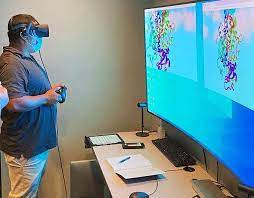
\includegraphics[width=0.5\textwidth]{img/vlab2}
		      \caption{Simulateur scientifique EON RealityC}
		      \label{fig:mesh1}
	      \end{figure}
\end{itemize}

\begin{table}[H]
    \centering
    \caption{Comparatif des solutions existantes}
	\begin{tabular}{|l|p{5cm}|p{5cm}|}
		\hline
		\textbf{Application}       & \textbf{Avantages}                                                                                      & \textbf{Inconvénants}                                                          \\ \hline
		ONTOP DUO MEAC             & Très immercif et réaliste, maintenu et populaire dans le milieu de l'aviation.                          & Trop chère pour une utilisation à domicile, pas adapté aux sciences chimiques. \\ \hline
		Microsoft flight simulator & Assez peu chère à l'obtention donc adapté à une utilisation à domicile et maintenu                      & Pas tres immercif et réaliste, pas adapté aux science chimiques                \\ \hline
		Osso VR                    & Immercif, assez réaliste et maintenu                                                                    & Disponible seulement en démo, pas adapté aux science chimiques.                \\ \hline
		Praxilab                   & Assez réaliste, accessible, adapté au expérience chimique et maintenu                                   & Pas tres immercif, impossible de creer des réactions, pas de version francaise \\ \hline
		EON Reality                & immercif, tres polyvalent, disponible sur de nombreuses plateformes et en plusieurs langues et maintenu & impossible de creer des réactions                                              \\ \hline
	\end{tabular}
\end{table}

\subsubsection{Questions de recherche}

\begin{itemize}
    \item Comment pouvons nous rendre l'enseignement de la chimie moins couteux ?
    \item Comment pouvons nous rendre l'enseignement de la chimie moins risqué ?
    \item Comment concerver l'aspect réaliste et immercif des expérimentations réelles ?
    \item Comment permettre aux enseignants de creer des réactions pour leur expérimentations ?
\end{itemize}